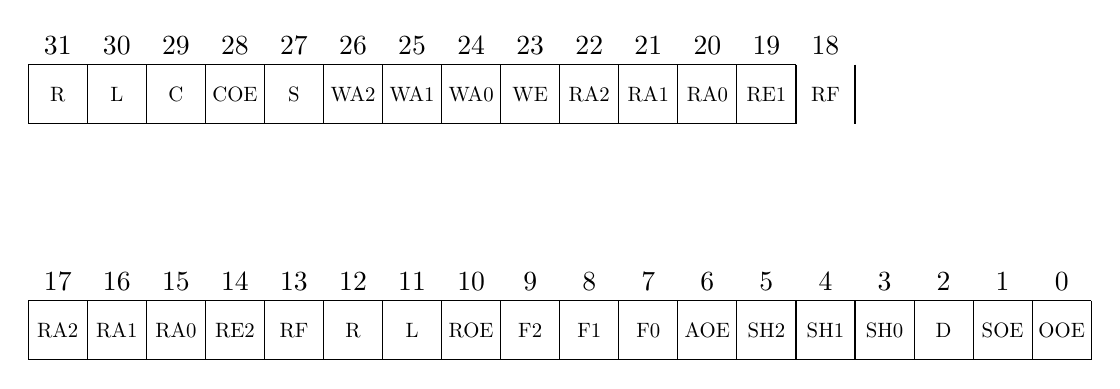
\begin{tikzpicture}
\foreach \j/\xa/\xb/\b in {0/31/19/{31/R,30/L,29/C,28/COE,27/S,26/WA2,25/WA1,24/WA0,23/WE,22/RA2,21/RA1,20/RA0,19/RE1,18/RF},-3/17/0/{17/RA2,16/RA1,15/RA0,14/RE2,13/RF,12/R,11/L,10/ROE,9/F2,8/F1,7/F0,6/AOE,5/SH2,4/SH1,3/SH0,2/D,1/SOE,0/OOE}} {
  \begin{scope}[yshift=\j cm]
  \foreach \i/\t in \b {
	%\begin{scope}
	\coordinate (X) at (0.75*\xa-0.75*\i,0);
	\coordinate (XN) at (0.75*\xa-0.75*\i,0.375);
	\coordinate (XA) at (0.75*\xa-0.75*\i+0.375,0);
	\coordinate (XAN) at (0.75*\xa-0.75*\i+0.375,0.375);
	\node[scale=0.75] (I-\i) at (X) {\t};
	\draw (XAN) -- ++(0,-0.75);
	\draw (XN) node[anchor=south] {$\i$};
	%\end{scope}
  }
  \draw (0.75*\xa-0.75*\xb+0.375,0.375) -- (-0.375,0.375) -- (-0.375,-0.375) -- (0.75*\xa-0.75*\xb+0.375,-0.375);
  \end{scope}
}
\end{tikzpicture}